\documentclass{bmvc2k}
\usepackage{graphicx}
\usepackage{amsmath}
\usepackage{amssymb}
\usepackage{mathtools} % mathtools builds on and extends amsmath package
\usepackage{algorithm}		% http://ctan.org/pkg/algorithms
\usepackage{algpseudocode}	% http://ctan.org/pkg/algorithmicx% Include other packages here, before hyperref.
\usepackage{comment, url}
%% Enter your paper number here for the review copy
\bmvcreviewcopy{825}

\title{ {\it E}nKCF: Ensemble of Kernelized Correlation Filters for Object Tracking in High Speed}

% Enter the paper's authors in order
% \addauthor{Name}{email/homepage}{INSTITUTION_CODE}
\addauthor{Susan Student}{http://www.vision.inst.ac.uk/~ss}{1}
\addauthor{Petra Prof}{http://www.vision.inst.ac.uk/~pp}{1}
\addauthor{Colin Collaborator}{colin@collaborators.com}{2}

% Enter the institutions
% \addinstitution{Name\\Address}
\addinstitution{
 The Vision Institute\\
 University of Borsetshire\\
 Wimbleham, UK
}
\addinstitution{
 Collaborators, Inc.\\
 123 Park Avenue,\\
 New York, USA
}

\runninghead{Student, Prof, Collaborator}{BMVC Author Guidelines}

% Any macro definitions you would like to include
% These are not defined in the style file, because they don't begin
% with \bmva, so they might conflict with the user's own macros.
% The \bmvaOneDot macro adds a full stop unless there is one in the
% text already.
\def\eg{\emph{e.g}\bmvaOneDot}
\def\Eg{\emph{E.g}\bmvaOneDot}
\def\etal{\emph{et al}\bmvaOneDot}

%-------------------------------------------------------------------------
% Document starts here
\begin{document}

\maketitle

%%%%%%%%% ABSTRACT
\begin{abstract}
Computer vision technologies are very attractive for practical
applications for embedded systems. This is primarily because most of
the embedded systems already includes image acquisition pipeline and a
tremendous amount of progresses on research has been made for many
areas in computer vision. However, to successfully deploy a computer
vision algorithm on any existing embedded systems, a vision algorithm
needs to satisfy some criteria: minimal, manual intervention after
deployment and small footprint of computing resource consumption and
on executable code, with the assumption of reasonably good
performance. To this end, in this paper, we propose an ensemble of the
kernelized correlation filters (KCF), we call {\it E}nKCF, for a
single-target object tracking. In particular, we developed a committee
of KCFs to specifically address the scale-change and dynamic maneuver
of the target over frames. In addition, we devised a Bayes filter for
a smooth transition between individual KCFs' executions. To minimize
the effect of drifting, we also developed another algorithm that
detects target-lost, uses an existing object proposal method (e.g.,
``Edge Box'') to re-detect the lost target, and re-initializes the
previous tracking for a long-term tracking. To verify the usefulness
of the proposed method, we compared the performance of ours to those
of the existing online tracking methods. Experimental results showed
that the performance of ours are 72.53\% for precision on 20 pixels
and 52.90\% for success rate for OTB100 data, and 55.71\% and 41.71\%
for UAV123 data. These results confirmed that our method outperformed
the existing ones over 5\% on precision on 20 pixels and 10-20\% on
AUC on average. Our implementation ran at 340 fps for OTB100 and at
416 fps for UAV123 data that is faster than DCF (292 fps) for OTB100
and KCF (292 fps), DCF (457 fps), and STC (350 fps) for UAV123.
\end{abstract}

%%%%%%%%% BODY TEXT
\section{Introduction}
\begin{comment}
\begin{itemize}
\item YoungWoo: Clean up the introduction
\item Burak: Clean up the technical section: EnKCF, KCF, and Particle Filter
\item Burak: You'll have a conclusion whether we'll have the re-detection part by Friday night.
\item By Monday, we'll have a draft ready to submit.
\end{itemize}
\end{comment}
A recent proliferation of air/ground/water unmanned vehicle
technologies has ever increased interests on deploying intelligent
algorithms on embedded or mobile platforms. Among those technologies,
computer vision algorithms are getting more attentions primarily
because payloads of those mobile platforms are limited to carry any
other sensors than a lightweight or an array of monocular cameras. For
example, instead of having just bare flight function with video
recording, an unmanned air vehicle (UAV) equipped with an object or
feature following functionality would make it more useful in the
application of monitoring/surveillance/surveying on private
properties/wild-life/crop, video recording on sports/movies/events,
many others.

In this paper, we propose a single-target tracking aiming at running
on any embedded or mobile platforms that doesn't require an offline
training, and can run on an embedded system. In particular, we would
like to make our algorithm 1) learn the appearance model of a target
on the fly and 2) run as fast on a typical desktop as up to 300Hz so
that it could run, at least, faster than 30Hz when it is deployed on a
low-end, embedded system. With these features, our tracking algorithm
is ready to track an object of interest when it is deployed on an
embedded system. To this end, an online object tracking is more
appropriate.

One of the dominant frameworks for online object tracking is the
correlation filter that essentially solves a single-target tracking
problem as a regression problem in the frequency domain. This
framework assumes that the target location is given at the very first
image frame like other online tracking algorithms
\cite{smeulders2014survey}. Given this positive example for the
regression problem, a set of negative examples is collected around the
initial, target bounding box and represented as a circulant matrix
\cite{henriques2015high}. One can optimally solve this regression
problem using a ridge regression in a closed form. However, such a
solution involves in expensive matrix operations
$\mathcal{O}(n^{3})$. The correlation filter offers a less complex
solution, $\mathcal{O}(n\log n)$ over element-wise multiplication in a
frequecny domain \cite{bolme2010visual,henriques2015high}. Thank to
this reformulation, an object tracking pipeline based on the
correlation filter can be easily implemented and run very efficiently
in an online fashion. In fact, a variant of the correlation filter,
the kernelized correlation filter with multi-channel features
\cite{henriques2015high} showed impressive object trackin results and
outperformed other state-of-the-art tracking algorithms, for example,
in VOT15 challenge, in terms of run-time and tracking
accuracy. However, the vanilla form of such an online tracker is prone
to drift, and fails to track a target over a long period of time
primarily \cite{henriques2015high} because of the dilemma of
stability-plasticity in updating appearance model, where the
appearance model will be overfitted to only the images used to train
and a compromise on the frequency of updating the model is carefully
implemented \cite{santner2010prost}. For example, a naive way of
handling a scale change of a target could reduce the run-time
performance from 300 to 100 fps. A seemingly obvious way of addressing
the scale change is to scan the region of interest (ROI) with
templates in different dimensions based on pre-defined scale ratios to
find the target
\cite{henriques2015high,tang2015multi,ma2015long,bibi2015multi,li2014scale}. Due
to the computational nature of correlation filter, however, this
approach would merely increase the computational complexity because it
has to run the correlation filter multiple times on each frame.

Another way of handling the scale change for the correlation filter
based approach is to find a correct scale at a location where a target
highly likely appears \cite{zhang2014fast}. In particular, they uses
the MOSSE tracker to estimate a target's translation. The scale is
updated in a way where the confidence map is used to determine the
scale change between successive frames. This is because they assumes
the scale of a target wouldn't change much over two consecutive
frames. Similarly \cite{ma2015long} used two KCFs to learn the
translation and scale of a target separately. To more specific, a KCF
is used to learn the translation of the target and its
background. Given this, another KCF is used to learn the target area
to estimate a new scale of the target. However, because of running
more than a KCF on each frame, this method degrades its run-time
performance (i.e., $\leq 50 fps$). Our method is motivated by this
idea -- the idea of deploying multiple KCFs to address the issues of
single target tracking: scale and translation. In this paper, we use
an ensemble of KCFs in turn, instead of running them all together on
every frame. By doing so, we could still address the scale change and
estimate target's motion efficiently while increasing run-time
performance. In particular, we deploy three KCF in turn:
\textit{target}+\textit{small background} translation filter
($R_{t}^{S}$), \textit{target-only} scale filter ($R_{s}$) and
\textit{target}+\textit{large background} translation filter
($R_{t}^{L}$). Figure \ref{fig:Filters} shows examples of the ROIs
associated with $R_{t}^{S}$, $R_{t}^{L}$, and $R_{s}$.
\begin{comment}
{\it We may not need this.}
The recent progress on development of convolutional neural networks
(CNN) is astonishing as since the AlexNet \cite{krizhevsky12} broke
the record for the ImageNet competition, at every year, new and better
results are reported. Moreover, there have been many attempts to
deploy CNN on the mobile devices
\cite{wu2016quantized,giusti2015}. But the inherent limitation of such
a supervised learning based object tracking is that an either online
\cite{nam2016} or offline \cite{held2016} training tracker has to be
prior to deploy the algorithm.
\end{comment}

The contributions of this study are as follows.
\begin{itemize}
\item \textbf{Novel Single-Target Tracking in a Very High-Speed} Our
  algorithm, {\it E}nKCF, deploys an ensemble of KCF in turn to more
  efficiently address the scale variance and the dynamic maneuver of a
  target while perserving run-time performance as high as possible. To
  minimize any potential performance gap from transiting one KCF to
  another, we use a Bayes filter. The workflow of the  {\it E}nKCF can
  be visualized in fig.~\ref{Workflow_figure}. 

\item \textbf{Re-Detection} A target loss is inevitable in object
  tracking. To cope with this, we developed a new target, re-detection
  that reliably detects when to lose the target and effectively
  re-detect the lost target. {\it How we can show how good our
    re-detection method is?}

\begin{comment}
\item We build a highly efficient ($\geq300$ fps) scale adaptive
  multiple kernelized correlation filter based tracker that
  outperforms the original KCF implementation with fixed scale
  framework both in terms of accuracy and performance. The studies
  following the KCF improved the fixed scale framework by running
  detection on a number of candidate ROIs to figure out the new scale
  of the object after estimating the translation of the object. This
  approach adds additional complexity to the original KCF
  implementation and drags down the run-time performance from $300$
  fps to less than $100$ fps.

\item We integrate the Particle Filter into the Multiple KCFs tracking
  as an additional filter that can avoid the drift due to one of the
  correlation filters we employ in our framework.

\item We propose a target re-detection module that can minimize the
  target loss due to the scale filter that learns the object model
  using only-object area. Also, the target re-detection step is
  required to handle severe occlusions, pose variations, illumination
  changes and fast motion.

\item Since our visual tracker mostly focuses on tracking objects from
  aerial moving platforms, we design a new robust target-to-camera
  distance estimation method. This way, a safe distance between the
  target and the camera-platform can be preserved.
\end{comment}

\end{itemize}

%---------------------------------------------------------------------- 
\section{{\it E}nKCF: Ensemble of Kernelized Correlation Filters}
%---------------------------------------------------------------------- 

\begin{figure*}[!t]
\includegraphics[width=\textwidth]{figures/Workflow_MKCF+PF.pdf}
\caption{The workflow of the proposed {\it E}nKCF with a particle filter.}
\label{Workflow_figure}
\end{figure*}

In this paper, we extends the KCF in that multiple KCFs are deployed,
in turn, to address a target's scale change and dynamic maneuvers
while preserving the overall execution time very fast, i.e., $\ge$ 300
fps. The efficient nature of KCF computation results in a
small-footprint, executable. Such a fast execution will facilitate to
deploy the proposed algorithm on any embedded systems.

The proposed algorithm, {\it E}nKCF, deploys three KCFs in turn: The
first filter, $R_{t}^{S}$, focuses on learning the target area and its
background, \textit{target}+\textit{small background} for addressing a
marginal translation by a target, the second filter, $R_{s}$, focuses
entirely on learning the target's scale, \textit{target-only}, and the
last filter, $R_{t}^{L}$, focuses on the target area and its
background twice bigger than that of the first filter, $R_{t}^{S}$,
\textit{target}+\textit{large background}. We set up {\it E}nKCF in
this way because we believe a correlation filter for learning a
target's translation should include its background to better
discriminate the target from its background and another correlation
filter is prepared to focus on the target itself to estimate the right
size or scale of the target. Figure \ref{fig:Filters} shows examples
of the region of interest (ROI) covered by each of three filters. We
believe that a filter for learning a target's translation should
include its background. In addition, making the ROI for the scale
filter, $R_{s}$, tighter reduces the size of the template for the
elementwise multiplication, resulting in a scale estimation in a
higher speed.

After Heriques and his colleagues' presented impressive tracking
results of KCF \cite{henriques2015high}, many variation of KCF were
investigated. In particular, \cite{ma2015long} and
\cite{danelljan2014accurate} used a scale filter to learn the target
area only whereas \cite{li2014scale, bibi2015multi, tang2015multi}
used a correlation filter learned on the target area and its
surrounding background in different size to learn the optimal scale of
the target. Our approach is particularly similar to that of
\cite{ma2015long} in that more than one KCF is used to address the
challenges of single target tracking. But ours is different from that
of \cite{ma2015long} in that we do not use those three KCFs together
at every frame, but alternatively at every three frame. The way our
algorithm is alternating multiple KCFs in different goals intuitively
makes sense in that the appearance of consecutive images does not
change much. Although it varies based on the scene, learning a
correlation filter a frame would not be much different from the one
learned using the image few or $k$ frames later. By alternating three
KCFs in turn, our algorithm runs as fast as or faster than the
original KCF. From our experiments, we empirically found that five is
the optimal for $k$ in terms of precision and success rates. We'll
detail this at the experimental section later.

\begin{figure}[!t]
\centering
\includegraphics[width=0.5\textwidth]{figures/Filters_Details.pdf}
\caption{The three filters denoted as \textit{target+small background} translation filter,
  \textit{target-only} scale filter and \textit{target+large background} translation filters are
  shown. Also, the hanning window and desired Gaussian response for
  each filter is displayed.}
\label{fig:Filters}
\end{figure}

The order of deploying these three KCFs is {\it Burak: Answer this}

The \textit{target+large background} translation filter, $R_{t}^{L}$,
is designed to run in right next frame after the scale filter,
$R_s$. We deploy these two filters in this way because we want to
minimize any drifts, which are likely to happen running only $R_{s}$.


{\it Burak: Rewrite the following two sentences.}

Considering a large ROI for $R_{t}^{L}$ can degrade its performance
due to information loss resulting from ROI resizing.

On the other hand, only HoG features are used in $R_{t}^{S}$ as it
focuses on a smaller ROI, giving us more discriminative HoG
features. 

The reason why our {\it E}nKCF comes with two KCF for translation {\it
  Burak: Answer this.}

In our framework, $R_{t}^{S}$ addresses the absence of scale
adaptation module in $R_{t}^{L}$ and $R_{t}^{S}$ whereas $R_{t}^{L}$
focuses on addressing the absence of translation estimation module in
$R_{S}$. 


$R_{t}^{S}$, on the other hand, focuses on the shape features
of the target that is not fully exploited in $R_{t}^{L}$ and
$R_{t}^{S}$. For this reason, we employ \textit{HoG} features in
$R_{t}^{S}$ and \textit{HoG} and \textit{Color} features in
$R_{t}^{L}$. Fig.~\ref{Workflow_figure} displays the proposed tracking
framework called Ensemble of KCFs {\it E}nKC. Also, the pseudo-code of
the proposed {\it E}nKC is shown in alg.~\ref{alg:MKCF}.

\begin{algorithm}
	\caption{The EnKCF Tracking Algorithm.}\label{alg:MKCF}
	\begin{algorithmic}[1]
	\State \textbf{Input} : Initial bounding box $x_{0}$, frame counter $fc$, scale filter frequency $n = 5$,
	\State \textbf{Output} : 
				\If{$fc\:\%\:n=0$} \Comment{Condition 1}
						\State Estimated Target State $x_{t} = (x_{t-1},y_{t-1},s_{t})$,
						Scale filter (\textit{target-only}) model $R_{s}$.
			     \EndIf
				\If{$fc\:\%\:n=1\:\:or\:\:fc\:\%\:n=2$}\Comment{Condition 2}
						\State Estimated Target State $x_{t} = (x_{t},y_{t},s_{t_1})$,
						Large Area Translation Filter model $R_{t}^{L}$.
				\EndIf
				\If{$fc\:\%\:n=1\:\:or\:\:fc\:\%\:n=4$}\Comment{Condition 3}
						\State Estimated Target State $x_{t} = (x_{t},y_{t},s_{t})$,
						Small Area Translation Filter model $R_{t}^{S}$.
				\EndIf
	\Procedure{track}{$x_{t-1},y_{t-1},s_{t-1}$} 
				\State // Translation Estimation
				\State Transit Particle Filter to the frame $t$ and compute the mean of prior pdf $x_{t} = (x_{t},y_{t},s_{t-1})$;
				\State // Translation Estimation
				\State Crop the ROI for the $R_{t}^{L}$, or $R_{t}^{S}$ given $x_{t}$
				and estimate translation ($x_{t}$,$y_{t}$) using $R_{t}^{L}$ (Condition 2) or $R_{t}^{S}$ (Condition 3),
				\State Skip translation estimation for $R_{s}$ (Condition 1);
				\State // Scale Estimation
			    \State Crop the ROI for the $R_{s}$ and estimate scale, $s_{t}$, using $R_{s}$ (Condition 1), 
		         \State Skip it for $R_{t}^{L}$ (Condition 1),
				\State Scale pool for $R_{s}$ : $\lbrace1.05,1.0,1/1.05\rbrace$;
				\State // Update Translation
				\State Perform Importance Re-sampling for Particle Filter and compute the mean of posterior pdf $x_{t} = (x_{t},y_{t},s_{t})$;
			    \State // Model Update
				\If{$PSR(y_{R_{s}}) \geq T_{R_{s}}$}
				\State Update $R_{s}$ (Condition 1);
				\EndIf							 
				\If{$PSR(y_{R_{t}^{L}}) \geq T_{R_{t}^{L}}$} 
				\State Update $R_{t}^{L}$ (Condition 2);
				\EndIf	
			     \If{$PSR(y_{R_{t}^{S}}) \geq T_{R_{t}^{S}}$}
				\State Update $R_{t}^{S}$ (Condition 3);
			     \EndIf		
	\EndProcedure	
	\end{algorithmic}
\end{algorithm}

\subsection{Kernelized Correlation Filter} \label{sec:kcf}
The Kernelized Correlation Filter tracker has recently been
increasingly popular due to its operation at hundreds of frames per
second with state-of-the-art tracking capabilities even in challenging
cases such as VOT15 dataset. Its computational efficiency arises from
its use of the discrete fourier transform of the circulant matrix and
frequency domain element-wise operations known as hadamard product and
division. The first example of frequency domain trackers is the Linear
Correlation Filter tracker known as MOSSE tracker. It minimizes the
ridge regression function in the frequency domain using a single
template with continous desired gaussian response. The KCF tracker, on
the other hand, minimizes the regularized ridge regression function
shown below.
\begin{equation}
E(h) = \frac{1}{2}||y-\sum_{c=1}^{C}h_{c}*x_{c}||^{2} + \frac{\lambda}{2}\sum_{c=1}^{C}||h_{c}||^{2}
\label{eq:Closedform_RidgeReg}
\end{equation}
where $y$ represents the desired continous response whereas $h$ and
$x_{c}$ represents the learned correlation filter and training
template for the given channel. The $c$ parameter included in
\cite{henriques2015high,galoogahi2013multi} makes it possible to
integrate multi-channel features such as HoG and colour into the ridge
regression function. The closed-form solution for the
eq.~\ref{eq:Closedform_RidgeReg} can be obtained by setting the
derivative of $E$ w.r.t $w$ to $0$. The solution in the primal domain
can be formulated as
\begin{equation}
w = (X^{T}X+\lambda)^{-1}y
\label{eq:SpatialSolution}
\end{equation}
where $X$ and $\lambda$ represent the training samples and
regularization term. The same cost function in the Fourier domain can
be represented as
\begin{equation}
w = (X^{H}X+\lambda I)^{-1}X^{T}y
\label{eq:FourierSolution}
\end{equation}
More information on the spatial and fourier domain solutions can be
found in \cite{henriques2015high}. The MOSSE tracker does not make use
of $\lambda$ and only one training sample with desired response is
used to update $w$. This framework does not include enough background
information into the training framework with a single template. The
application of the circulant matrix theorem into the
eq.~\ref{eq:Closedform_RidgeReg} makes it possible to include many
background patches at a similar computational complexity. A circulant
matrix includes the circularly shifted patches of the positive
training sample $x$ by a cylic shift operator. 

%By applying shifting operation to the base sample, we can generate the circulant
%matrix as
%\begin{equation}
%C = Px.
%\label{eq:CirculantMatrixGeneration}
%\end{equation}
%The circulant matrix of a base sample $x$ can be interpreted as the
%rows of a training matrix $X$ where each row represents features of a
%training sample. Mathematically, this can be written as
%\begin{equation}
%X = C(x)
%\label{eq:CIrculantMatrixTrainingData}
%\end{equation}

In this form, eq.~\ref{eq:SpatialSolution}
and~\ref{eq:FourierSolution} could prohibit us from implementing a
high speed object tracking as we need to perform large number of
element-wise division and multiplication operations. However, we know
from \cite{gray2006toeplitz} that all circulant matrices are
represented diagonally by the Fourier Transform regardless of the base
sample $x$ as shown below.
\begin{equation}
X = Fdiag(\hat{x})F^{H},
\label{eq:CirculantMatrixDFT}
\end{equation}
where $F$ denotes a constant Fourier Transform matrix and $x$ is the
Discrete Fourier Transform of the base sample $x$. 
%To simplify the
%cost function formulation in eq.~\ref{eq:FourierSolution} we multiply
%$X$ in eq.~\ref{eq:CirculantMatrixDFT} with $X^{H}$ yielding
%\begin{equation}
%X^{H}X = Fdiag(\hat{x}^{*}\odot \hat{x})F^{H}.
%\label{eq:SimplificationX} 
%\end{equation}
The solution vector in the Fourier domain $\hat{w}$ is formulated as
\begin{equation}
\hat{w} = \dfrac{\hat{x}^{*}*\hat{y}}{\hat{x}^{*}*\hat{x}+\lambda}.
\label{eq:DiagonalizedPrimalSolution}
\end{equation}
For detailed documentation of the circulant matrix theorem based
frequency domain solution can be found in
\cite{henriques2012exploiting,henriques2015high}.

The above primal frequency domain solution can be called as Linear
Correlation Filter which improves the MOSSE tracker by incorporating
cyclic shifts and regularizer. To further improve the robustness to
geometric and photographic variations, one can exploit non-linear
regression function in the Correlation Filter framework
\cite{henriques2015high}. The solution to the kernelized ridge
regression function is shown below.
\begin{equation}
\alpha = y(K+\lambda I)^{-1},
\end{equation}
where $K$ and $\alpha$ represent the kernel matrix and corresponding
dual space solution. 

%\cite{henriques2015high} states that kernel
%matrices is circulant for datasets of circular cylic satisfying the
%following theorem.
%\begin{equation}
%k(x,x^{'}) = k(Mx,Mx^{'}),
%\label{eq:KernelCirculantTheorem}
%\end{equation}
%where $M$ represents the permutation matrix. Some kernels satisfying
%the eq.~\ref{eq:KernelCirculantTheorem} are \textit{Gaussian},
%\textit{Polynomial}, \textit{Intersection} and \textit{Hellinger}
%kernels. 

Similar to the diagonalization in the linear ridge regression
solution in eq.~\ref{eq:DiagonalizedPrimalSolution}, the kernelized
ridge regression can be made diagonal using the same circulant matrix
theorem.  The diagonalized Fourier domain dual form solution can be
expressed as
\begin{equation}
\hat{\alpha} = \hat{y}(\hat{k}^{xx}+\lambda)^{-1}
\label{eq:FourierDualDomainSolution}.
\end{equation}
where $\hat{k}^{xx}$ represents the first row of the Kernel matrix $K$
known as \textit{gram matrix}. In this study, we will only focus on
application of the Gaussian Kernel to the Correlation Filters. We
refer the readers to \cite{henriques2015high} for the detailed
documentation of the application of other kernels to the Correlation
Filters. The Gaussian kernelization is
expressed as
\begin{equation}
k^{xx^{'}} = exp(-\dfrac{1}{\alpha^{2}}(||x||^{2}+||x^{'}||^{2}-2F^{-1}(\sum^{C}_{c}\hat{x}_{c}^{*}\odot \hat{x}_{c}^{'}))).
\label{eq:GaussianCorrelationSingleChannel}
\end{equation}
%\begin{equation}
%k^{xx^{'}} = exp(-\dfrac{1}{\alpha^{2}}(||x||^{2}+||x^{'}||^{2}-2F^{-1}(\hat{x}^{*}\odot \hat{x}^{'})))
%\label{eq:GaussianCorrelationSingleChannel}
%\end{equation}
The first correlation filter based trackers used grayscale feature ($C=1$) to
learn the solution vector $w$, however, the multi-channel features
such as HoG and Color were later exploited to improve tracking
accuracy \cite{henriques2015high,galoogahi2013multi,tang2015multi,ma2015long,bibi2015multi}. The
multi-channel feature integration into the Gaussian Kernelization
function in eq.~\ref{eq:GaussianCorrelationSingleChannel} is achieved
in a very straight-forward way by summing the correlation result over the channels.

Such non-linearization process does not increase the computational
complexity of the linear multi-channel correlation filter dramatically
as we only need to sum over the $n$ dimensional feature
channels. Training shown in eq.~\ref{eq:FourierDualDomainSolution}
gives us $\hat{a}$ learned in time step $t$. We can accumulate
$\hat{a}$ over time to integrate more temporal information. This can
be expressed as
\begin{equation}
\hat{a}_{t} = (1-\beta)\hat{a}_{t-1} + \beta\hat{a}_{t}. 
\end{equation}

Finally, detection step in multi-channel KCF framework is performed as
\begin{equation}
r(z) = F^{-1}(\hat{k}^{xz} \odot \hat{\alpha})
\end{equation}
where $r$ denotes the correlation response at all cylic shifts of the
first row of the kernel matrix $K$. The peak point of the response
function gives us the estimated translation of the object from time
step $t$-$1$ to $t$.

\subsection{Particle Filter} \label{sc:PF}
The proposed MKCF algorithm can cause undesired drift and noise in
tracking due to independent application of the correlation filters. To
mitigate the drift effect and reduce the noise, a Bayes Filter
representing the evolution of target's motion can be added into the
MKCF tracking framework. In this study, we consider a variant of a
Bayes Filter, \textit{Particle Filter}. The Particle Filter is a
Sequential Monte Carlo method that can approximate posterior
probability density functions (pdf) of a target motion. The
approximation becomes optimal with the infinite number of particles,
however, its run-time complexity grows exponentially with the number
of elements in the state space matrix, $X_{t}$. As the focus of this
study is to design a high speed tracker, we keep the number of state
space elements low and implement computationally cheap \textit{Weight
  Function} and \textit{Importance-Resampling} modules. We represent
the state space matrix as $X_{t} = \lbrace x,y,V_{x},V_{y}\rbrace$
where $x$ and $y$ are the centroid of the target and $V$ represents
the velocity components. We transit the particles with the well-known
first order Constant Velocity model. The centroid components are
applied Gaussian Noise whereas the velocity components are assigned
uniform noise representative of most of the objects. The observation
likelihood is modeled based on the confidence map of
$R_{t}^{L}$,$R_{t}^{S}$, and $R_{s}$. It can also be modeled based on
the euclidean distance between particle's centroid to the peak of the
confidence maps, however, we believe that the former approach could
result in further drifts in the case of multi-modal distributions. The
weights for the particles are computed with the bilinear interpolation
method.
\begin{equation}
	w_{p_{t}}(x_{t},y_{t}) = \dfrac{y_{R}(x_{t}-1,y_{t}-1)+y_{R}(x_{t}+1,y_{t}+1){y_{R}(x_{t}+1,y_{t}-1)+y_{R}(x_{t}-1,y_{t}+1)}}{4}
\end{equation}
where $w_{p}$ denotes the weight of the particle. The importance
re-sampling module is triggered when the number of effective particles
is smaller than a pre-defined threshold [Cite - Effective Number
  Samples Metric] to avoid variance getting too small. Re-sampling is
implemented with highly efficient low-variance ratio method
[cite]. Finally, the expected mean of the approximated posterior pdf
is computed as
\begin{equation}
	\hat{X}_{t} = \sum_{p=1}^{P}w_{p_{t}} X_{t}
\end{equation}

The particles are assigned equal weight ($\dfrac{1}{P}$) after the
importance re-sampling step. It should be emphasized that we skip
importance re-sampling step in the scale filter operation as the scale
filter contains \textit{target-only} area. In this case, the particles
outside of the scale filter ROI do not have weight correspondence in
the confidence map. Also, it is more likely to get noisy translation
estimation from the scale filter.

%----------------------------------------------------------------------
\section{Experiments} \label{sc:Experiments}
%---------------------------------------------------------------------- 
To verify the usefulness of our algorithm, we ran the proposed
algorithm against two publicly, available datasets:
OTB100 \footnote{\url{http://cvlab.hanyang.ac.kr/tracker_benchmark/benchmark_v10.html}},
UAV123 \footnote{\url{https://ivul.kaust.edu.sa/Pages/Dataset-UAV123.aspx}}\cite{mueller2016uav123}. OTB100
dataset contains video sequences for 100 objects whereas UAV123
dataset contains aerial footage of 123 objects. 

The proposed $E$nKCF method can better handle slow motions. Also, the
UAVs use mobiles platforms with limited computational power. We
believe that the proposed tracker can better fit to tracking from
these platforms as it is highly efficient and scale adaptive. Taking
into account these reasons, it is more appropriate to test it on
aerial videos captured by UAVs.

\textbf{Hyperparameter Selections.} Tuning the hyper-parameters of the
committee of the correlation filters are important as the each
correlation filter addresses the weakness of another one. For
instance, $R_{t}^{L}$'s main task is to recover from the previous
frame where only $R_{s}$ and particle filter's prior distribution are
used to estimate scale and translation. We set the learning rates
($\beta$) of $R_{t}^{L}$, $R_{t}^{S}$, and $R_{s}$ as $0.020$, $0.020$
and $0.010$. The desired response and hanning window for each KCF is
shown in fig.~\ref{fig:Filters}. Finally, the Gaussian kernel
parameter, $\alpha$ is tuned to $0.6$, $0.4$, and $0.4$ for
$R_{t}^{L}$, $R_{t}^{S}$, and $R_{s}$. In our particle filter
implementation, we employ $1000$ particles and use the
\textit{efficient number of samples} metric shown below to determine
whether we need to perform importance re-sampling or not to keep
reasonable variance.
\begin{equation}
  \hat{N}_{eff} = \dfrac{1}{\sum_{i=1}^{P}(w_{p})^{2}}, 
\end{equation}
 where $w$ represents the particles' weights and re-sampling is performed only if $\hat{N}_{eff}$ is smaller than three.

\textbf{Features Selections.} We use the fast Histogram of Oriented
Gradients (fHoG)\cite{felzenszwalb2010object} and
Color-naming\cite{van2009learning} features to learn target and
background models. $R_{t}^{L}$ uses both fHoG and color features as it
covers a large ROI where fHoG features may not be reliable alone. On
the other hand, $R_{t}^{S}$ is assigned only fHoG features as it
covers smaller ROI. Finally, $R_{s}$ uses both fHoG and color features
as it is assigned lower template size, yielding space to exploit two
feature modalities.

\begin{figure}
\centering
\begin{tabular}{cc}
\bmvaHangBox{\includegraphics[width=4.00cm]{./figures/Precision_UAV123.pdf}}
\bmvaHangBox{\includegraphics[width=4.0cm]{./figures/Success_UAV123.pdf}}\\
\end{tabular}
\caption{Evaluation and comparison of the proposed E$n$KCF tracker on the UAV123 dataset. UAV123 Dataset consists of $123$ video sequences captured from a micro UAV including large camera motion, low resolution objects, partial and full occlusions. Our tracker better fits to tracking from aerial platforms as the scale change in successive frames are not dramatic.}
\label{fig:UAV123_DATASET}
\end{figure}

\begin{figure}
\centering
\begin{tabular}{cc}
\bmvaHangBox{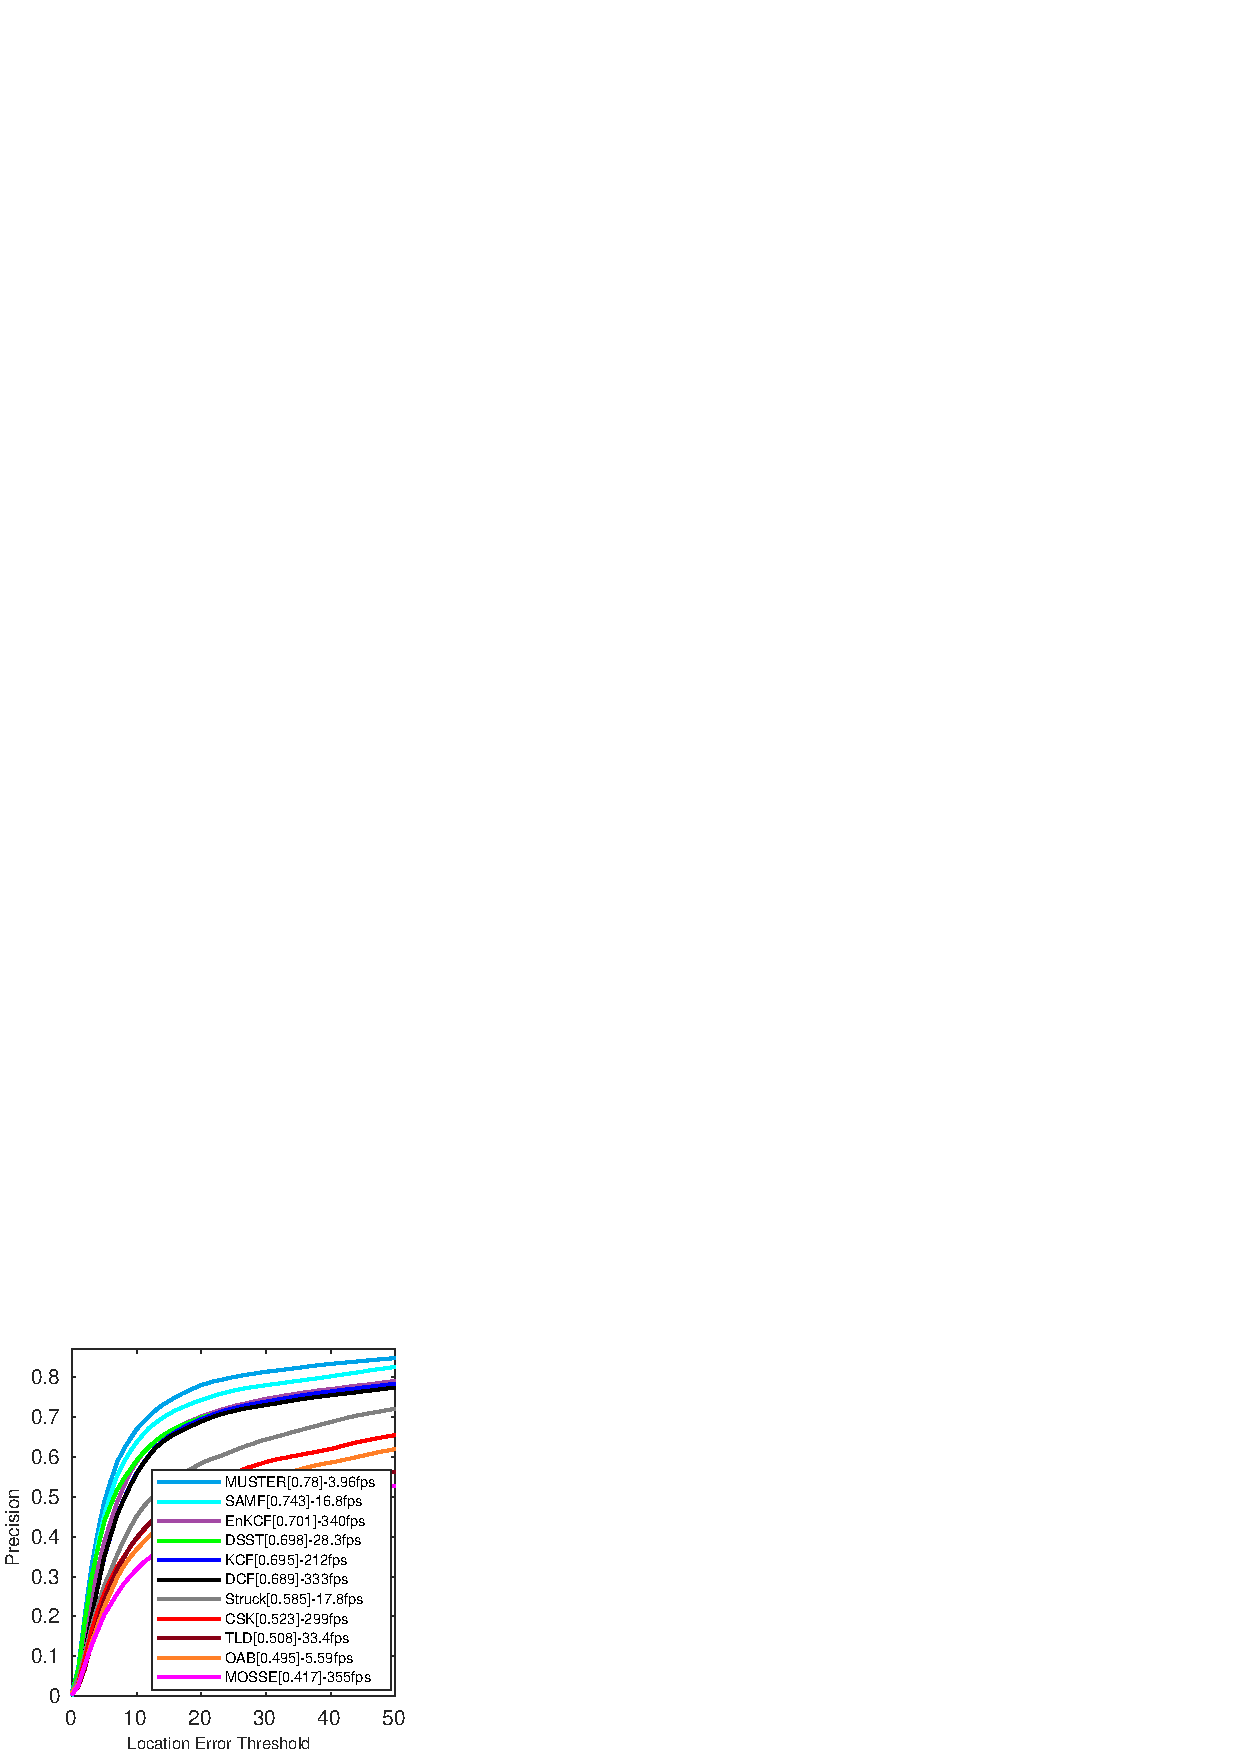
\includegraphics[width=4.00cm]{./figures/Precision_OTB100.pdf}}
\bmvaHangBox{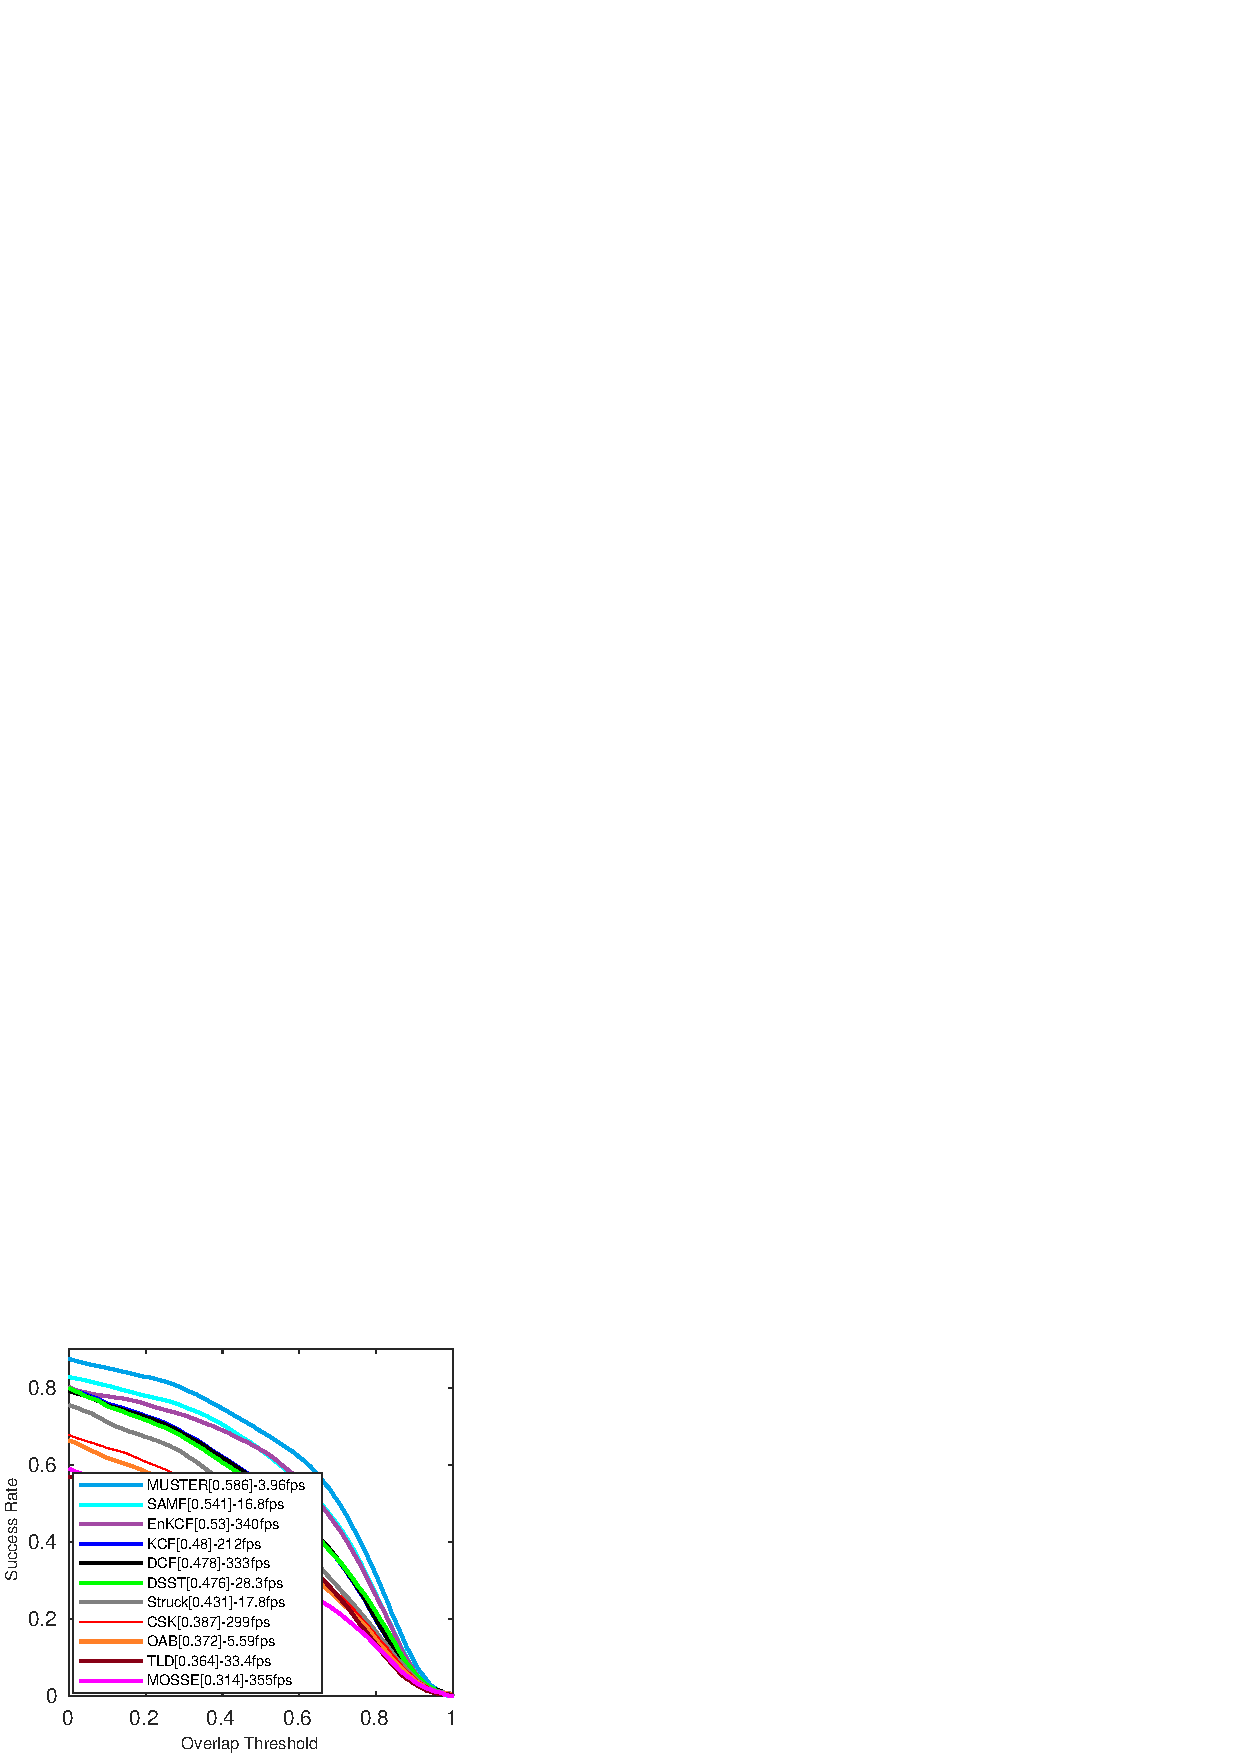
\includegraphics[width=4.0cm]{./figures/Success_OTB100.pdf}}\\
\end{tabular}
\caption{Evaluation and comparison of the proposed E$n$KCF tracker on the OTB100 dataset. OTB100 dataset consists of $100$ video sequences of different objects from recent literatures.}
\label{fig:OTB100_DATASET}
\end{figure}
%\begin{figure}
%        \begin{subfigure}{0.5\textwidth}
%                \includegraphics[width=\linewidth]{./figures/Precision_UAV123.pdf}
%        \end{subfigure}%
%        \begin{subfigure}{0.5\textwidth}
%                \includegraphics[width=\linewidth]{./figures/Success_UAV123.pdf}
%        \end{subfigure}%
%        \caption{Evaluation and comparison of the proposed E$n$KCF tracker on the UAV123 dataset. UAV123 Dataset consists of $123$ video sequences captured from a micro UAV including large camera motion, low resolution objects, partial and full occlusions. Our tracker better fits to tracking from aerial platforms as the scale change in successive frames are not dramatic.}\label{fig:UAV123_DATASET}
%\end{figure}
%
%\begin{figure}
%        \begin{subfigure}{0.5\textwidth}
%                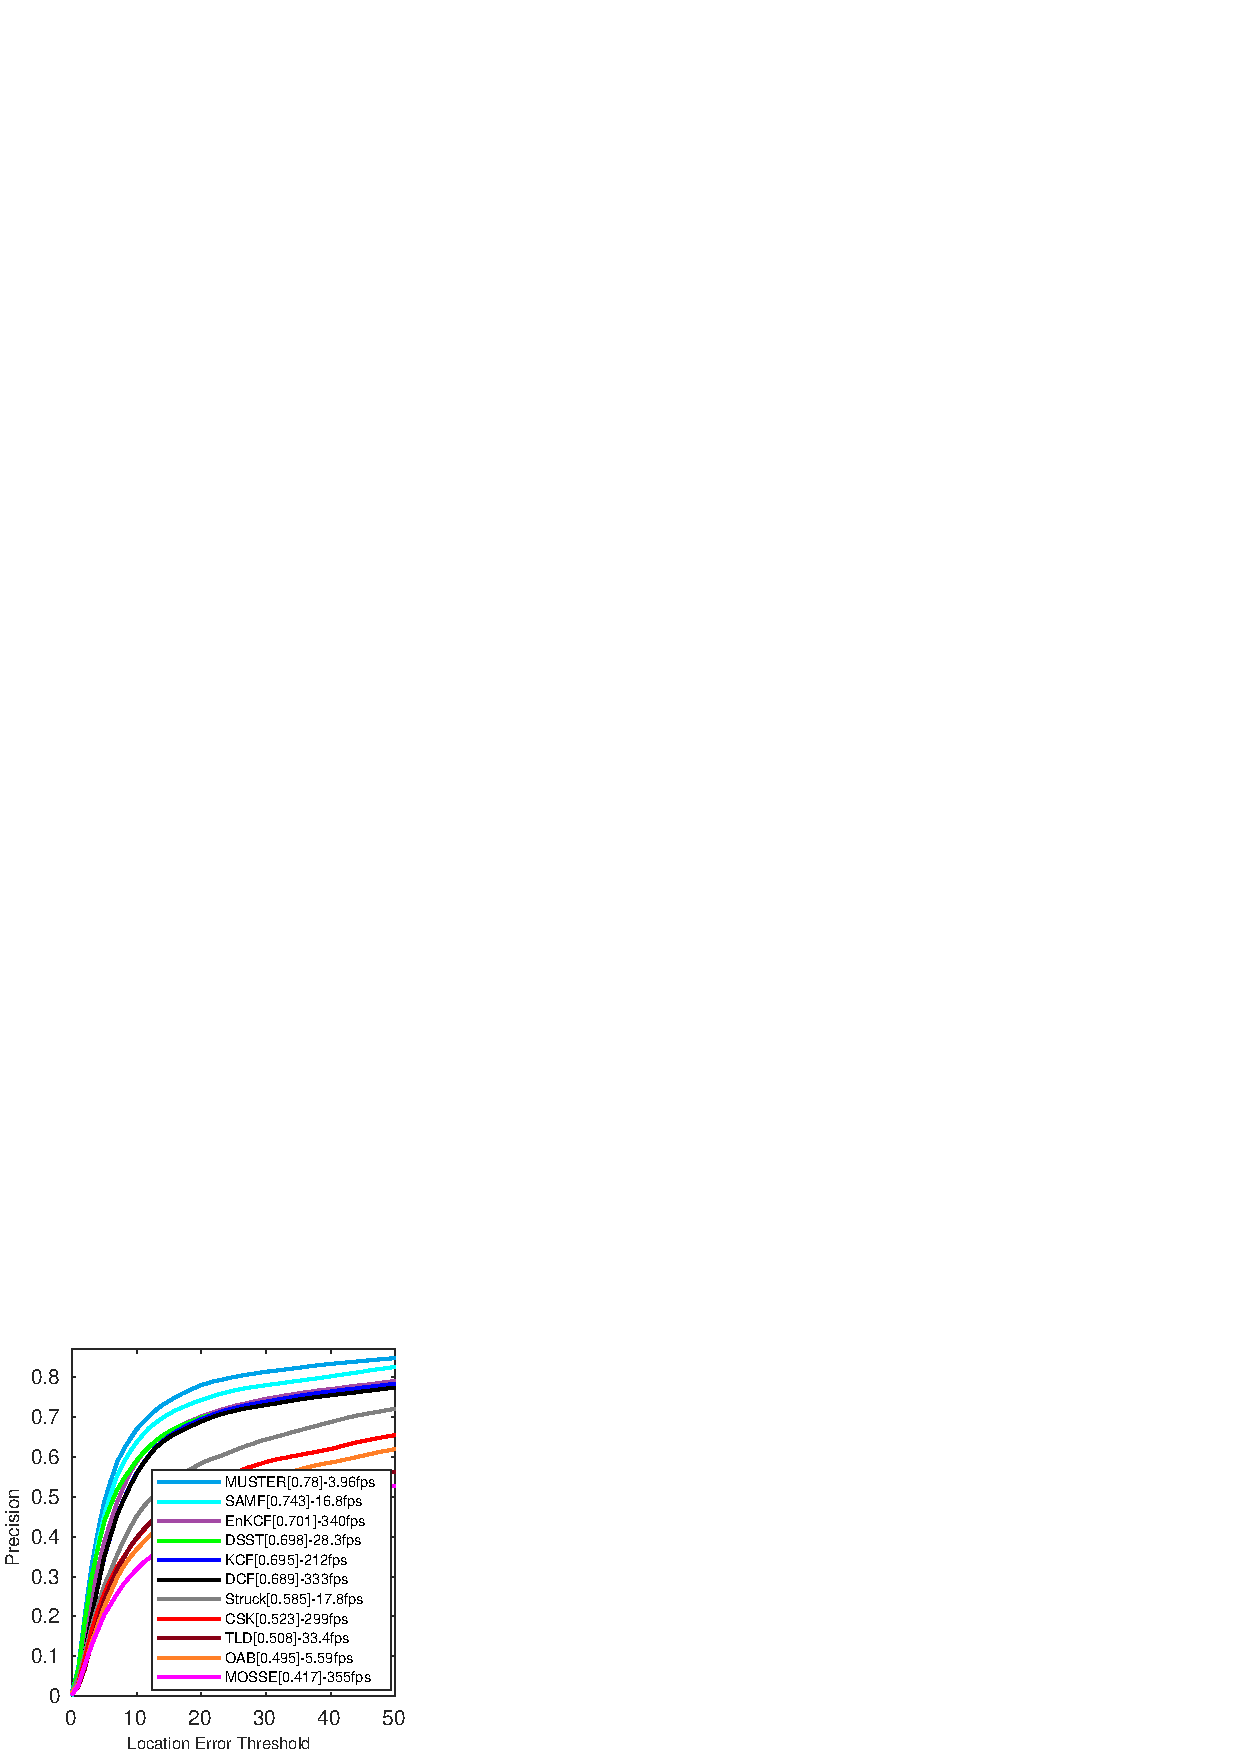
\includegraphics[width=\linewidth]{./figures/Precision_OTB100.pdf}
%        \end{subfigure}%
%        \begin{subfigure}{0.5\textwidth}
%                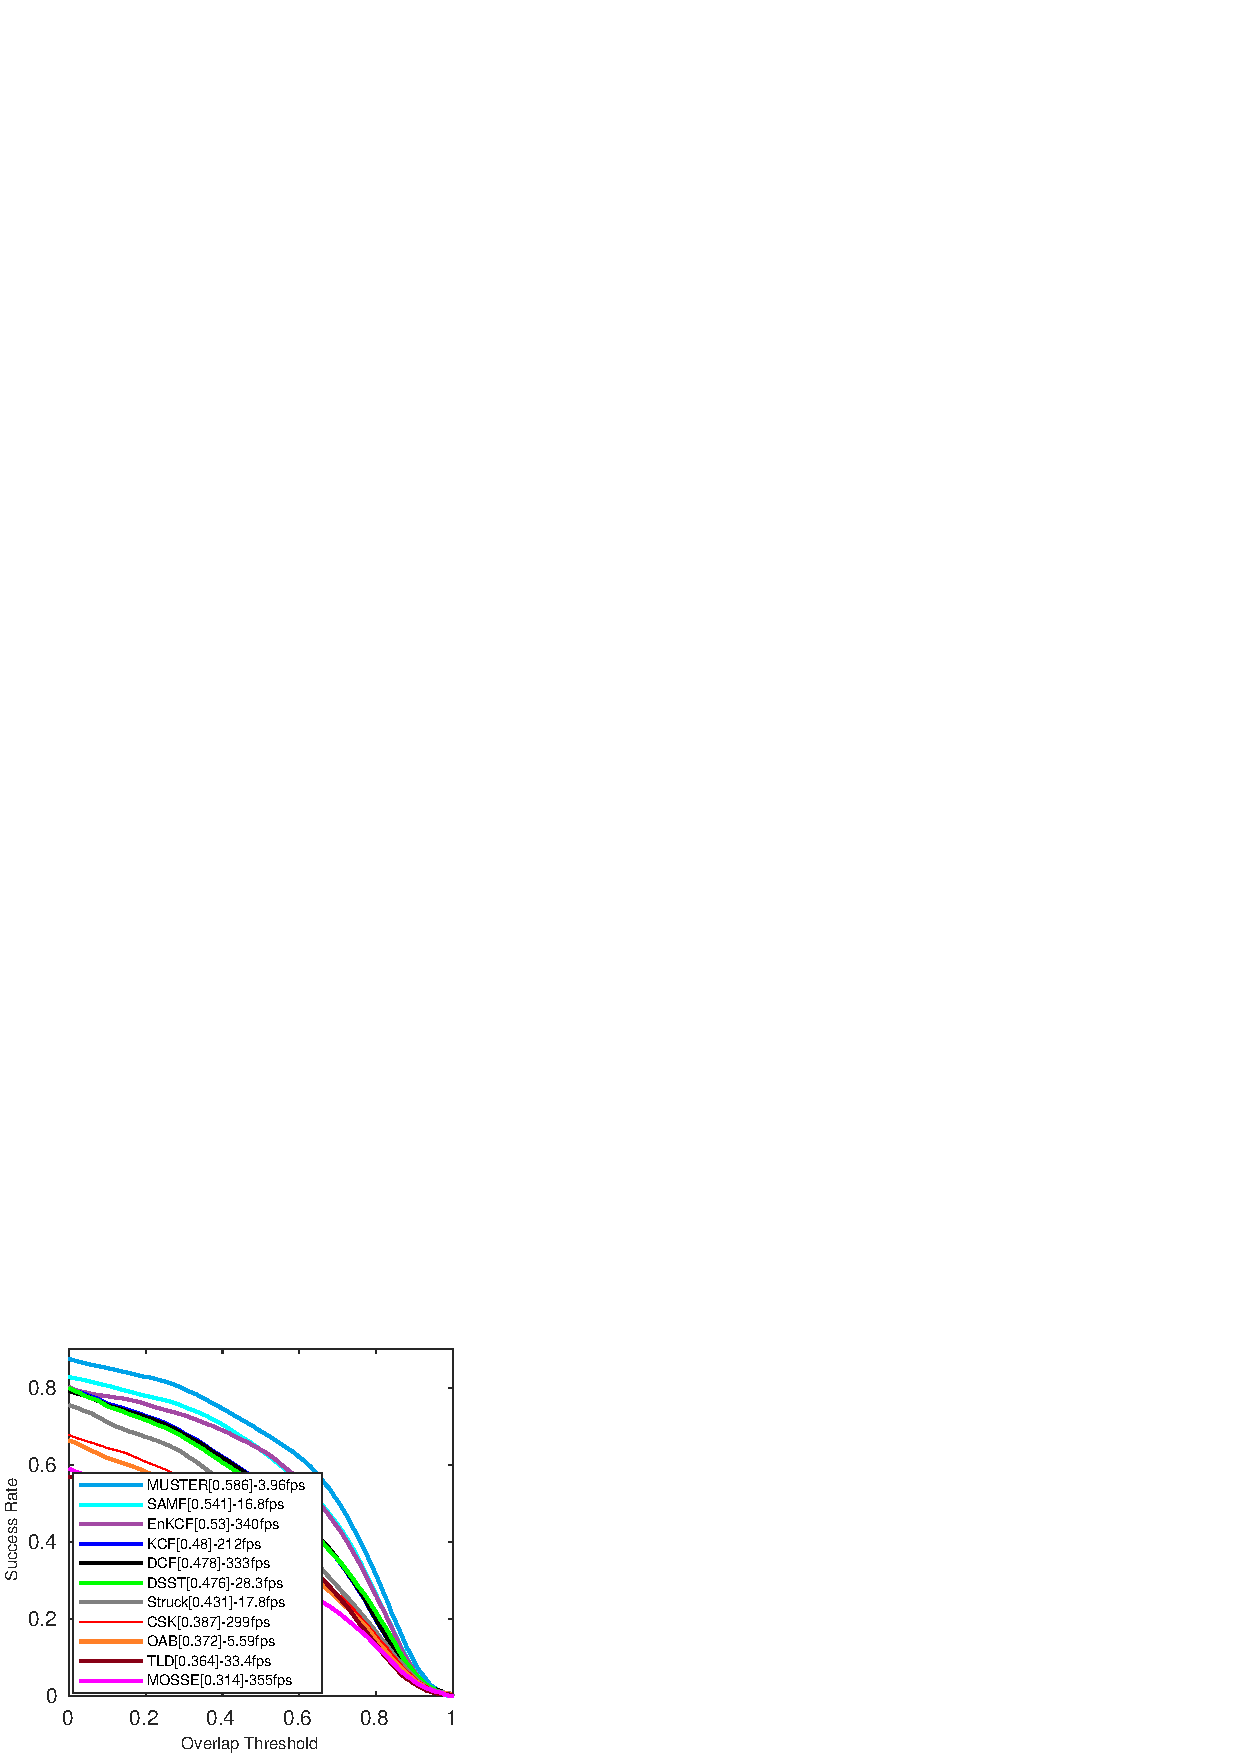
\includegraphics[width=\linewidth]{./figures/Success_OTB100.pdf}
%        \end{subfigure}%
%        \caption{Evaluation and comparison of the proposed E$n$KCF tracker on the OTB100 dataset. OTB100 dataset consists of $100$ video sequences of different objects from recent literatures. }\label{fig:OTB100_DATASET}
%\end{figure}

\textbf{Overall Performance without Re-detection on UAV123 Dataset.}
We compare the proposed tracker to other state-of-the-art high speed
trackers using the \textit{Precision} and \textit{Success\:Rate}
metrics. Precision is computed by thresholding the average euclidean
distance between the ground truth and tracking output over the frames
of one sequence. In precision, we rank the trackers based on the
precision numbers at 20 pixels. The success rate metric evaluates the
overlap between the ground truth and tracking output. The
intersection-to-union ratio of two regions over the frames of one
sequence. Finally, we count the number of frames with overlap larger
than the success rate threshold and divide it by the number of
frames. We compare our tracker to some other high-speed ($\geq$300
fps) state-of-the-art trackers including KCF\cite{henriques2015high},
CSK \cite{henriques2012exploiting}, STC\cite{zhang2014fast},
MOSSE\cite{bolme2010visual,henriques2015high}. Also, some relatively
lower-speed ($\geq$50) trackers are used to evaluate the robustness of
the proposed trackers. These trackers include SAMF\cite{li2014scale},
DSST\cite{danelljan2014accurate}, LCT\cite{ma2015long},
MEEM\cite{zhang2014meem} and Struck\cite{hare2012efficient}.
Fig.~\ref{fig:UAV123_DATASET} shows the results on the UAV123
dataset. The E$n$KCF tracker outperforms the other methods in
high-speed trackers category by $3\%$-$15\%$ at 20 pixels precision
accuracy whereas it is only $5\%$ worse than SAMF, DSST and Struck on
the same dataset although it is $10$-$20$ times faster than these
trackers. On the other hand, the E$n$KCF does a decent job on
approximating the scale of the target in highly efficient manner. This
is proved by the fact that it ranks third best tracker in terms of
\textit{area under curve} (AUC) value for the success rate plot. It
outperforms the high speed trackers by about $20\%$-$25\%$ in AUC
metric. Interestingly, it performs even better than most of the low
speed trackers. For instance, it outperforms Struct and DSST by $5\%$
and $10\%$ while running at more than $30$ and $10$ times larger
operation rate.

\textbf{Overall Performance without Re-detection on OTB100 Dataset.}
In addition to UAV123 dataset, we test the E$n$KCF tracker on the
OTB100 dataset to evaluate how good it generalizes to a traditional
object tracking dataset. Again, it performs slightly better than the
high speed trackers in precision. Interestingly, it outperforms the
another correlation filter based tracker, DSST while running only
$5\%$ behind of another low-speed scale adaptive SAMF tracker. As in
UAV123 dataset, the E$n$KCF performs exceptionally in handling the
scale changes. It is ranked as the fifth best tracker while being the
second highest speed tracker behind MOSSE. It performs only around
$2\%$ worse than SAMF and MEEM trackers in terms of AUC. These numbers
prove that E$n$KCF is not only a good candidate for tracking on a
UAV-based mobile platform but also mobile platforms on smart phones.

%---------------------------------------------------------------------- 
\section{Conclusion} \label{sc:Conclusion}
%---------------------------------------------------------------------- 

%--------------
%\section*{Acknowledgements}
%put stuff here for the accepted , but not the ICCV version

\bibliography{draft}
\end{document}
